\documentclass{standalone}
\usepackage{tikz}

\usetikzlibrary{calc,shadows}


\begin{document}

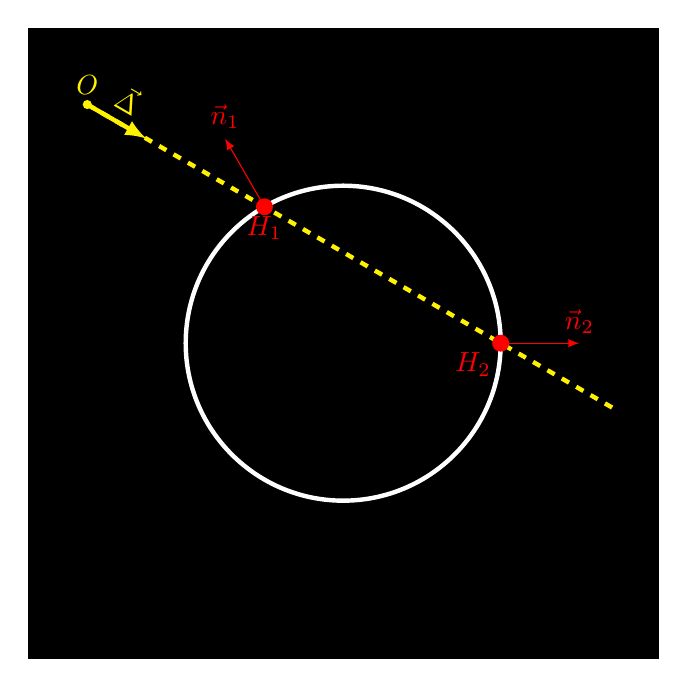
\begin{tikzpicture}
  \draw[fill=black,use as bounding box] (-4,-4) rectangle (4,4);
  \draw[white,ultra thick] (0,0) circle [radius=2cm];

  \coordinate (hit 1) at (120:2);
  \coordinate (hit 2) at (0:2);
  \coordinate (ray origin) at ($ (hit 1) ! -0.75 ! (hit 2) $);

  \draw[yellow,ultra thick,dashed] (ray origin) -- ($ (hit 1) ! 1.5 ! (hit 2) $);
  \draw[yellow,fill] (ray origin) circle [radius=0.05cm] node[above] {$O$};
  \draw[yellow,ultra thick,-latex] (ray origin) -- ($ (hit 1) ! -0.5 ! (hit 2) $) node[above,sloped,midway] {$\vec \Delta$};

  \draw[red,fill] (hit 1) circle [radius=0.1cm] node[anchor=north] {$H_1$};
  \draw[red,fill] (hit 2) circle [radius=0.1cm] node[anchor=north east] {$H_2$};

  \draw[red,-latex] (hit 1) -- ++(120:1) node[above] {$\vec n_1$};
  \draw[red,-latex] (hit 2) -- ++(0:1) node[above] {$\vec n_2$};
\end{tikzpicture}

\end{document}